% % % % % % % % % % % % % % % % % % % % % % % % % % % % % % % % % % % % % % % % % % % %
%                                                                                     %
% Short Sectioned Assignment LaTeX Template Version 1.0 (5/5/12)                      %
% This template has been downloaded from: http://www.LaTeXTemplates.com               %
%                                                                                     %
% Original author:  Frits Wenneker (http://www.howtotex.com)                          %
%                                                                                     %
% Modified by: Fco Javier Sueza Rodríguez (fcosueza@disroot.org)                      %
%                                                                                     %
% Changes:                                                                            %
%	    - Custom Chapters, Sections and Subsections (titlesec package)                %
%           - Document type scrbook (oneside)                                         %
%           - Use babel-lang-spanish package and marvosym                             %
%           - Use hyperref, enumitem, tcolorbox and glossaries packages               %
%           - Use Time New Roman (mathptmx), Helvetic and Courier fonts               %
%                                                                                     %
% License: CC BY-NC-SA 3.0 (http://creativecommons.org/licenses/by-nc-sa/3.0/)        %
%                                                                                     %
% % % % % % % % % % % % % % % % % % % % % % % % % % % % % % % % % % % % % % % % % % % %

%-----------------------------------------------%
%	              Packages                  %
%-----------------------------------------------%

\documentclass[paper=a4, fontsize=11pt, oneside]{scrbook}

% ---- Text Input/Output ----- %

\usepackage[T1]{fontenc}
\usepackage[utf8]{inputenc}
\usepackage{mathptmx}
\usepackage[scaled=.92]{helvet}
\usepackage{courier}
\usepackage[indent=12pt]{parskip}

\usepackage{geometry}
\geometry{verbose,tmargin=3cm,bmargin=3cm,lmargin=2.6cm,rmargin=2.6cm}

% ---- Language ----- %

\usepackage[spanish]{babel}
\usepackage{marvosym}

% ---- Another packages ---- %

\usepackage{amsmath,amsfonts,amsthm}
\usepackage{graphics,graphicx}
\usepackage{titlesec}
\usepackage{fancyhdr}
\usepackage{tcolorbox}
\usepackage{hyperref}
\usepackage{enumitem}
\usepackage[automake]{glossaries}

%--------------------------------------------------------------------%
%                      Customizing Document                          %
%--------------------------------------------------------------------%


% ----------- Custom Chapters, Sections and Subsections -------------- %

\titleformat{\chapter}[display]
			{\bfseries\Huge}
			{Tema \ \thechapter} {0.5ex}
			{\vspace{1ex}\centering}

\titleformat{\section}[hang]
			{\bfseries\Large}
			{\thesection}{0.5em}{}

\titleformat{\subsection}[hang]
			{\bfseries\large}
			{\thesubsection}{0.5em}{}

\titleformat{\subsubsection}[hang]
			{\bfseries\large}
			{\thesubsubsection}{0.5em}{}

\hypersetup{
    colorlinks=true,
    linkcolor=black,
    urlcolor=magenta
}

% ------------------- Custom heaaders and footers ------------------- %

\pagestyle{fancyplain}

\fancyhead[]{}
\fancyfoot[L]{}
\fancyfoot[C]{}
\fancyfoot[R]{\thepage}

\renewcommand{\headrulewidth}{0pt} % Remove header underlines
\renewcommand{\footrulewidth}{0pt} % Remove footer underlines

\setlength{\headheight}{13.6pt} % Customize the height of the header

% --------- Numbering equations, figures and tables ----------------- %

\numberwithin{equation}{section} % Number equations within sections
\numberwithin{figure}{section} % Number figures within sections
\numberwithin{table}{section} % Number tables within sections

% ------------------------ New Commands ----------------------------- %

\newcommand{\horrule}[1]{\rule{\linewidth}{#1}} % Create horizontal rule command


%----------------------------------------------------------------------------------------
%	TÍTULO Y DATOS DEL ALUMNO
%----------------------------------------------------------------------------------------

\title{
\vspace{10ex}
\normalfont \normalsize
\huge \textbf{Actividades de la Unidad 6: Medidas de Prevención y Protección}
}
\author{Francisco Javier Sueza Rodríguez}
\date{\normalsize\today}

%----------------------------------------------------------------------------------------
%                                     DOCUMENTO
%----------------------------------------------------------------------------------------
\begin{document}

\maketitle

\thispagestyle{empty}

\vspace{65ex}

\begin{center}
    \begin{tabular}{l l}
        \textbf{Centro}: & IES Aguadulce \\
        \textbf{Ciclo Formativo}: & Desarrollo Aplicaciones Web (Distancia)\\
        \textbf{Asignatura}: & Formación y Orientación Laboral\\
        \textbf{Tema}: & Tema 6: Medidas de Prevención y Protección\\
    \end{tabular}
\end{center}

\newpage

\tableofcontents

\newpage
\section{Caso Práctico}


Tras los numerosos incidentes  que estan ocurriendo últimamente en la empresa ``TECLASA'' y con la intención que estos no lleguen a convertirse en accidentes con daños para los trabajadores de la misma, la responsable y dueña decide reunirlos con el objeto de saber qué saben de prevención y protección en las tareas propias de su puestos de trabajo, aunque sea una empresa dedicada plenamente a la informática.

Marta observa y oye atónita los diferentes relatos de los trabajadores. Mario apila las cajas de folios y documentación que necesita en el suelo. Laura, su ubicación en el puesto de trabajo está tapando la salida de emergencia. Carla, que se dedica prácticamente a la programación no dispone de silla adecuada, ni reposapies y encima está al lado de la ventana donde le refleja toda la luz, ya que dice que ``le gusta que le de los rayos de sol en la cara''...en fin, todos y cada uno de los relatos y actuaciones de los mismos sólo hacen preocuparla mas todavía.

Decide poner manos a la obra, habla con la empresa que les lleva la prevención de riesgos con el objeto de que vengan a formarlos en la importancia de la prevención y protección de los riesgos a los que están expuestos, y a mentalizarlos que, aunque es una actividad que no es peligrosa, cualquiera puede en un momento dado estar expuesto a una situación de emergencia y, lo más importante, saber actuar frente a ella, además de los riesgos habituales de exposición.

Insiste con los técnicos en que no quiere algo teórico, y sí que lo realicen ``in situ'', para que no vuelva a caer en saco roto. La empresa de prevención se pone manos a la obra.

\section{Actividades}

\subsection{Actividad 1: Técnicas de prevención y medidas de protección}

\subsubsection{Enunciado}
\begin{enumerate}[label=\alph*.]
    \item Diferencia entre prevención y protección.
    \item Expón dos ejemplos de medidas de prevención y dos de protección.
    \item Define qué es la ergonomía aplicada como técnica en un puesto de Técnico Superior en Informática
    \item Aplica tres medidas ergonómicas que crees necesario aplicar en el puesto de tu perfil profesional.
    \item Respecto a los EPIs reflexiona y expón las reticencias e inconvenientes en que se basan las partes actoras de la relación laboral (empresariado y trabajadores) para su uso.
    \item Clasifica las medidas de protección y ejemplifica cada una de ellas.
\end{enumerate}

\subsubsection{Solución}
\begin{enumerate}[label=\alph*.]
    \item Las diferencias entre la prevención y la protección son:
    \begin{itemize}
        \item \textbf{Prevención}: se encarga de  \textbf{detectar}, \textbf{evaluar} y \textbf{eliminar} los riesgos laborales.
        \item \textbf{Protección}: en el caso de que haya \textbf{riesgos laborales} que no\textbf{ se hayan podido eliminar}, la protección se encarga de establecer \textbf{medidas para proteger} a los trabajadores y trabajadores de esos riesgos laborales.
    \end{itemize}
    \item Los ejemplos son los siguientes:
    \begin{itemize}
        \item \textbf{Medidas de Prevención}: dos ejemplos de medidas de prevención serían la \textbf{higiene industrial}, cuyo propósito es la prevención de enfermedades mediante el control de la presencia de agentes contaminantes y la \textbf{psicología aplicada}, destinada a prevenir y corregir  la insatisfacción laboral y el estrés.

        \item \textbf{Medidas de Protección}: por otro lado, dos ejemplos de medidas de protección serían, por un lado, \textbf{la señalización}, que consiste en el uso de señales visuales, luminosas o acústicas que alerten a los trabajadores de posibles riesgos, siendo ademas un ejemplo de \textbf{medidas de protección colectivas}. Por otro lado, un ejemplo de \textbf{medidas de protección individual} podría ser el \textbf{uso de EPIs}, que son los equipos de protección que debe llevar el trabajador para protegerse de uno o varios riesgos.
    \end{itemize}
    \item La \textbf{ergonomía} es el conjunto de técnicas y medias que intentan adecuar el puesto de trabajo al hombre, tratando de solucionar problemas que, aunque no daña la salud, pueden dar lugar a aparición de factores de carga, que causen fatiga, estrés, etc...

    Esto, \textbf{aplicado al puesto de Técnico Superior en Informática}, se traduce en la adecuación de puesto de trabajo, que suele ser un escritorio con uno o varios ordenadores, para que el trabajador este lo más cómodo posible, evitando malas posturas en la silla, problemas visuales por no tener una buena luminosidad, estrés por ruidos generados por impresoras u ordenadores, etc...

    \item Tres \textbf{medidas ergonómicas} que se podrían aplicar al puesto de Técnico Superior en Informático, y propuestas en la \textbf{Guía NTP 602} ``\textit{El diseño ergonómico del puesto de trabajo de pantallas de visualización}'' \cite{ntp602}, son las siguientes:
    \begin{itemize}
        \item Uso de \textbf{pantallas de panel plano}, ya que proporcionan mejores resultados en entornos con una iluminación mayor que las pantallas de rayos catódicos.
        \item Uso de \textbf{reposamuñecas}, que reduce la carga estática en los miembros superiores.
        \item Uso de \textbf{soporte del monitor} para poder regular el ángulo de visión y situar la pantalla en el ángulo más confortable para el usuario.
    \end{itemize}

    \item Respecto al uso de \textbf{EPIs}, tanto los empresarios como los trabajadores pueden tener sus reticencias, siendo estas:
    \begin{itemize}
        \item Los \textbf{trabajadores} pueden quejarse de que los equipos hacen que el trabajo sea menos ágil o de demasiada calor. Esto último puede verse, por ejemplo, en los trabajadores de la construcción, cuando realizan su labor en verano a altas temperaturas y elementos como el casco o los guantes pueden ser un extra de disconfort a la hora de realizar su labor.

        \item Por otro lado, \textbf{los empresarios}, se pueden quejar del gasto extra que supone la compra y mantenimiento de estos equipos.
    \end{itemize}
    \begin{itemize}
        \item
    \end{itemize}

    \item Las medidas de protección se pueden clasificar en:
    \begin{itemize}
        \item \textbf{Medidas de Protección Colectivas}: son aquellas encaminadas a proteger a todos los trabajador, teniendo mayor efectividad que las medidas de protección individuales. Un ejemplo sería el \textbf{uso de barandillas} para evitar la caídas de objetos a niveles inferiores.

        \item \textbf{Medidas de Protección Individuales}: son medidas encaminadas a proteger al trabajador individualmente, siendo las más empleadas, aunque solo debería hacerse cuando las medidas colectivas no sean suficientes. EL ejemplo más claro es el \textbf{uso de EPIs}, o \textbf{Equipos de Protección Individual}.
    \end{itemize}
\end{enumerate}

\subsection{Actividad 2: Señalización de Seguridad}

\subsubsection{Enunciado}
\begin{enumerate}[label=\alph*.]
    \item Haz una captura del artículo del Real Decreto sobre señalización de seguridad y salud en el trabajo en el que se define lo que se entiende por señalización de seguridad y salud en el trabajo.
    \item Cita los tipos de señales en forma de panel.
    \item Cita los otros tipos de señalización distintas a la de panel.
    \item Completa el siguiente texto extraído del  Anexo I del RD sobre señalización de seguridad y salud en el trabajo:
    ``\textit{La elección del tipo de señal y del número y emplazamiento de las señales o dispositivos de señalización a utilizar en cada caso se realizará de forma que la señalización resulte lo más eficaz posible, teniendo en cuenta: }''
\end{enumerate}

\subsubsection{Solución}
\begin{enumerate}[label=\alph*.]
    \item En la siguiente imagen, podemos ver una captura del \textbf{Real Decreto 485/1997} \cite{rd485}, la definición que se pide en concreto se encuentra en el \textbf{Artículo 2, Punto a}:

    \begin{figure}[H]
        \centering
        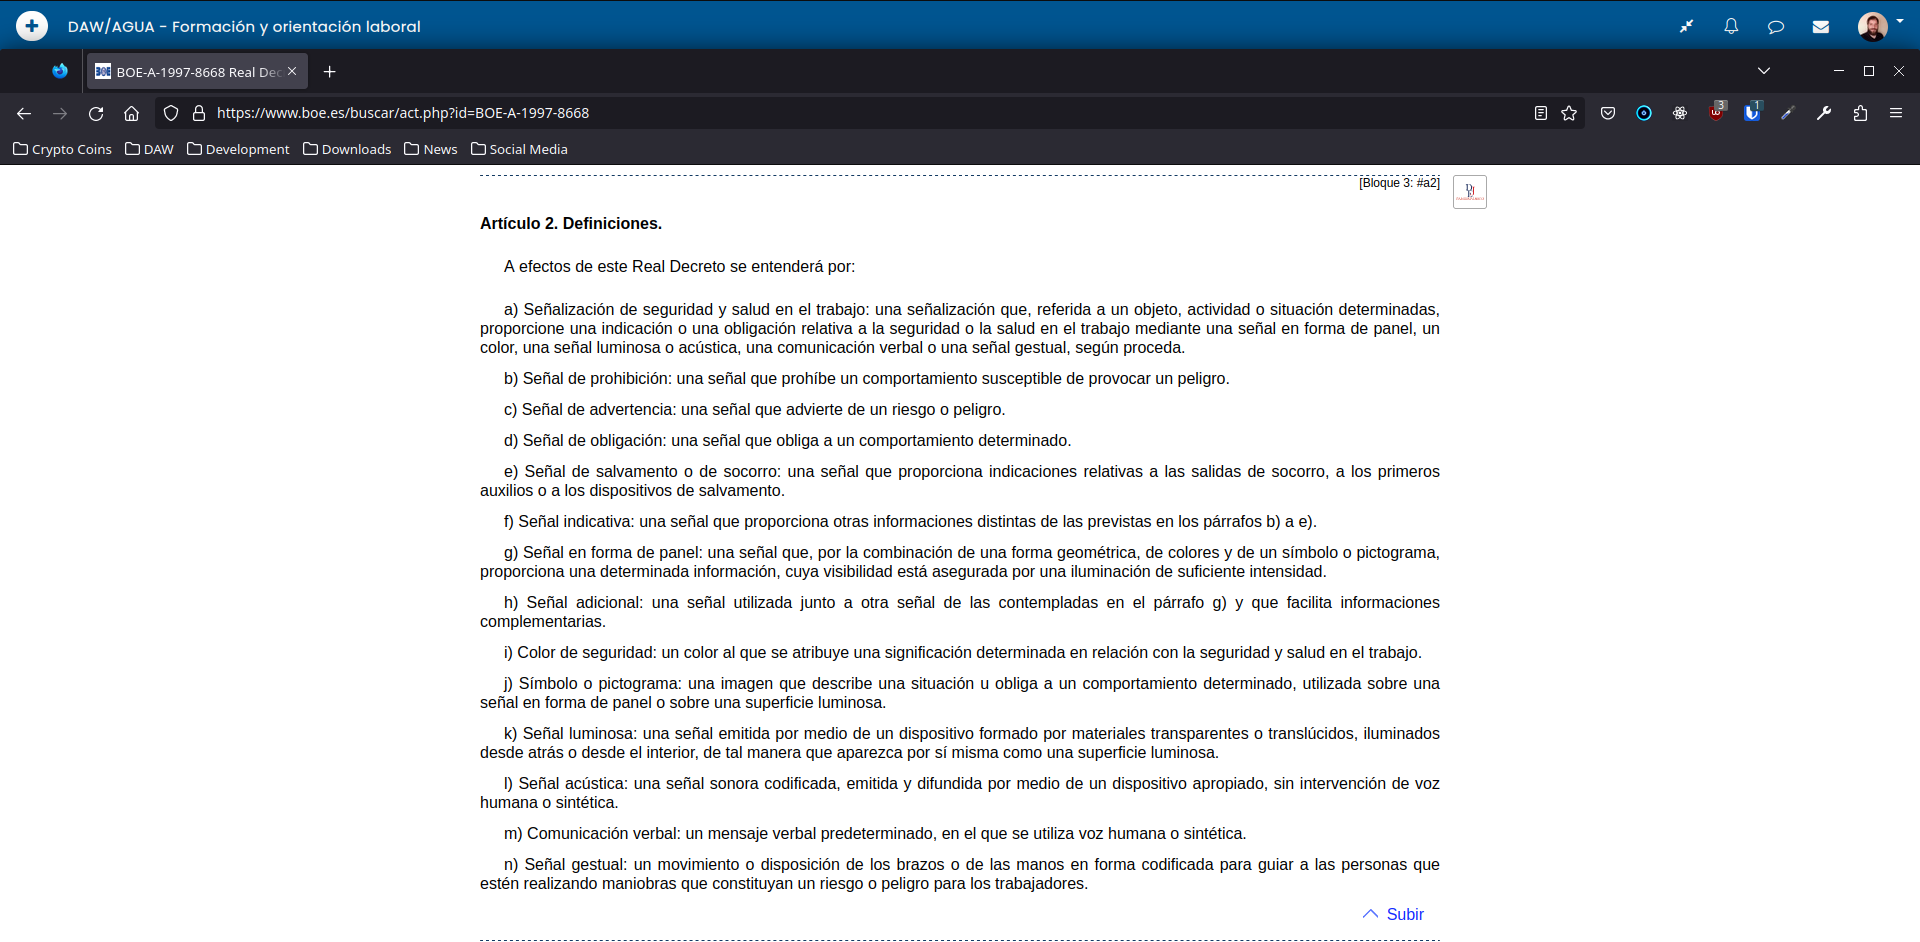
\includegraphics[scale=0.30]{real-decreto.png}
        \caption{Real Decreto 485/1997}
    \end{figure}

    \item Los \textbf{tipos de señalizaciones de panel} que nos podemos encontrar son los siguientes:
    \begin{itemize}
        \item \textbf{Prohibición}: Prohíbe un comportamiento determinado.
        \item \textbf{Obligación}: Obliga a un comportamiento determinado.
        \item \textbf{Advertencia}: Advierte de un riesgo o peligro.
        \item \textbf{Salvamento}: informa sobre las salidas de socorro, primeros auxilios o dispositivos de salvamento.
        \item \textbf{Indicativa}: proporciona otras informaciones.
    \end{itemize}

    \item Además de la señalización con paneles, podemos encontrarnos los siguientes tipos de señalización:
    \begin{itemize}
    \item \textbf{Señales Luminosa}: señal emitida por un dispositivo formado por materiales translucidos e iluminada desde atrás.
    \item \textbf{Señales Acústicas}: señal sonora codificada, difundida y emitida por un dispositivo apropiado.
    \item \textbf{Señales Verbales}: mensaje verbal predefinido donde usa una voz humana o sintética.
    \item \textbf{Señales Gestuales}: movimiento o disposición de los brazos o las manos de forma codificada para guiar  las personas que están haciendo alguna maniobra que entrañe riesgo.
    \item \textbf{Señales Olfativas}: son aditivos olorosos que se añaden a los gases tóxicos inodoros.
\end{itemize}
    \item La elección del tipo de señal y del número y emplazamiento de las señales o dispositivos de señalización a utilizar en cada caso se realizará de forma que la señalización resulte lo más eficaz posible, teniendo en cuenta:

    \begin{enumerate}[label=\alph*.]
        \item Las características de la señal.
        \item Los riesgos, elementos o circunstancias que hayan de señalizarse
        \item La extensión de la zona a cubrir
        \item El número de trabajadores afectados
    \end{enumerate}

    En cualquier caso, la señalización de los riesgos, elementos o circunstancias indicadas en el anexo VII se realizará según lo dispuesto en dicho anexo.
\end{enumerate}

\subsection{Actividad 3: Actuación ante situaciones de emergencia}

\subsubsection{Enunciado}
¿Crees necesario y conveniente realizar simulacros de emergencia en las empresas? Justifica, analiza y valora la misma.

\subsubsection{Solución}
En mi opinión, realizar \textbf{simulacros de emergencia} es algo \textbf{muy importante}.

En primer lugar, es una herramienta fundamental para valorar el plan de emergencia y comprobar su correcto funcionamiento. Mediante los simulacros, podemos medir los tiempos de evacuación, si las rutas de salida elegidas son las más óptimas, etc.. En resumen, nos sirve para realizar una evaluación eficaz del plan de emergencia y cambiar los elementos que haya que cambiar si fuera necesario.

Además, que los trabajadores conozcan dicho plan es algo que va a ayudar a la hora de producirse una emergencia, ya que van a saber que rutas deben tomar para realizar la evacuación y seguramente influya es que el proceso se realice con más tranquilidad por parte de éstos.

En conclusión, la realización de simulacros es necesaria y conveniente ya que no solo nos ayuda a valorar la eficiencia y los puntos flacos de nuestro plan de emergencia sino que ademas prepara a los trabajadores para una eventual emergencia.

\subsection{Actividad 4: Actuación ante situación de emergencia}

\subsubsection{Enunciado}
En situación de catástrofe en una empresa con múltiples víctimas el procedimiento a utilizar se denomina triage. Explica en qué consiste.

\subsubsection{Solución}
El \textbf{triaje} es un procedimiento empleado en situaciones de emergencia en las que hay múltiples victimas y que se usa para determinar el orden en el que hay que atender a estas víctimas. Esto se realiza por la persona que se ha desplazado al lugar de emergencia realizando un rápida valoración del estado de las diferentes víctimas. En la siguiente tabla, podemos ver un esquema de esa clasificación.

\begin{figure}[H]
    \centering
    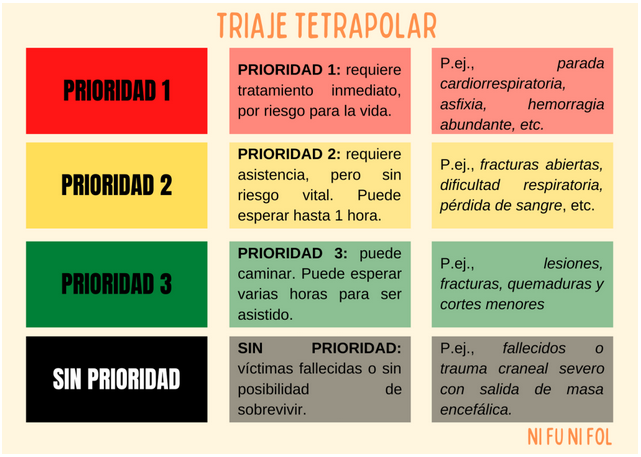
\includegraphics[scale=0.60]{triaje.png}
    \caption{Triaje tetrapolar}
\end{figure}

Uno de los métodos más empleados para establecer esta clasificación es el \textbf{método de traje SHORT}, que establece un algoritmo, determinando parámetros como si una víctima puede hablar, caminar, respira, etc...


\subsection{Actividad 5: Primero Auxilios}

\subsubsection{Enunciado}

\begin{enumerate}[label=\alph*.]
    \item Haz una captura en el que aparezca tu perfil de aula sobre alguna noticia  referente a primeros auxilios acontecida en este año 2022. Una vez subida al foro la captura añádela a la tarea y haz un comentario sobre ella y lo trabajado en el temario.
    \item Ante cualquier situación que nos encontremos en primeros auxilios debemos seguir tres pautas de conductas que se denomina PAS. Describe en que consiste y haz una valoración sobre la misma.
    \item ¿Crees necesario tener conocimientos sobre nociones básicas de primeros auxilios?
    \item Céntrate en alguna técnica o noción básica de primeros auxilios que crees necesaria, conveniente y muy recomendable que la persona trabajadora conozca o esté formada en ella.
\end{enumerate}

\subsubsection{Solución}

\begin{enumerate}[label=\alph*.]
    \item En la siguiente figura podemos ver la captura del foro de la unidad 5 con el mensaje posteado.

        \begin{figure}[H]
        \centering
        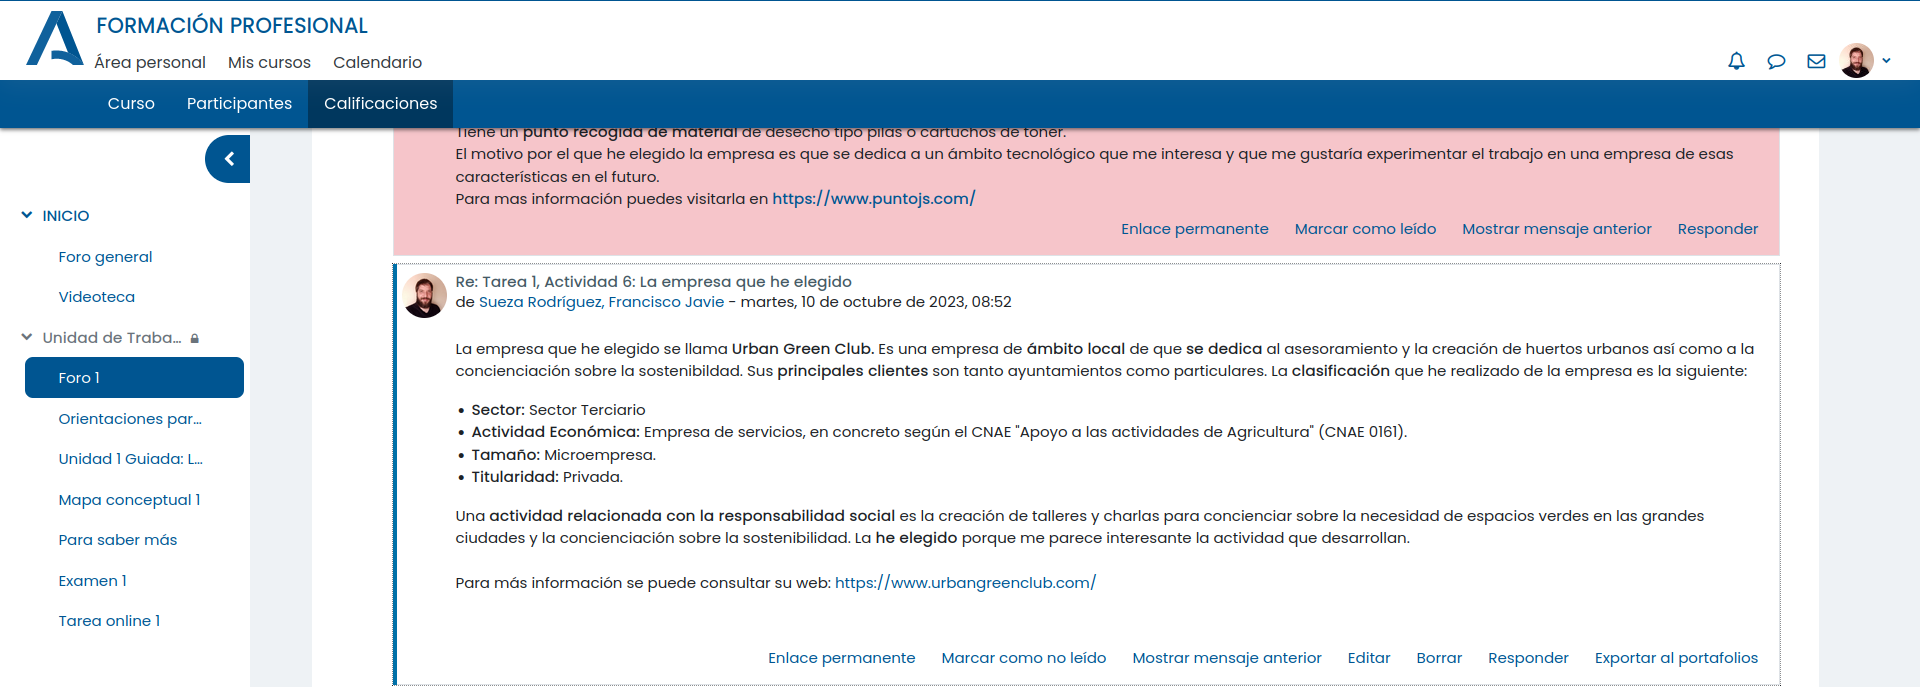
\includegraphics[scale=0.38]{captura-foro.png}
        \caption{Sección de Empleo Público del IAAP}
    \end{figure}

    \item Cuando estamos ante una emergencia, tenemos la obligación de socorrer a los afectados especialmente si están desamparados.  Para ello, debemos seguir la \textbf{conducta PAS} (Proteger, Alertar y Socorrer). Ahora pasamos a explicar cada una de las pautas de esta conducta:

    \begin{itemize}
        \item \textbf{Proteger}: lo primero de todo es \textbf{protegerse a uno mismo}, \textbf{a los accidentados} y a \textbf{terceras personas}. Por ejemplo, en caso de accidente se debe colocar el vehículo delante del accidentado para evitar más accidentes, en caso de una quemadura grave, se debe eliminar la causa o alejar a la persona afectada de ella, etc...

        Hay que tener en cuenta que si la zona no es segura tampoco debemos arriesgarnos y acabar siendo nosotros otra víctima del accidente.

        \item \textbf{Alertar}: el siguiente paso es \textbf{alertar a emergencia}, en nuestros caso \textbf{llamando 112}. Tenemos que tener clara cierta información para cuando hablemos con ellos, como que ha pasado, donde, quienes son los afectados, los peligros que hay y si están controlados o no, además de nuestros datos.

        \item \textbf{Socorrer}: en este punto es cuando debemos \textbf{realizar los primeros auxilios}, teniendo cuidado de no extralimitarse porque podría agravarse la situación de los accidentados.
    \end{itemize}
    \item Creo que tener conocimientos y formación básica en primeros auxilios es al \textbf{muy importante}, ya que es algo de mucha utilidad y que salva vidas si se aplica correctamente en determinadas circunstancias, por ello creo que debería ser parte de la formación que se imparte en los colegios e institutos desde los primeros años.

    \item La técnica de primeros auxilios en las que nos vamos a centrar es la \textbf{reanimación cardiopulmonar}, ya que considero que es una de las más importante, especialmente teniendo en cuenta que unas de las principales causas de muerte en España son las enfermedades cardiovasculares, incluidos los infartos.

    Esta técnica se compone de \textbf{3 pasos} que debemos realizar para su correcta aplicación. Estos son:

    \begin{enumerate}
        \item \textbf{Compresiones}: La compresiones significa que usaremos ambas manos para presionar con fuerza y de una manera específica sobre el pecho de la persona. Es uno de los pasos mas importantes de la reanimación. Hay que realizar la compresiones con las dos manos presionando el pecho de la persona a un ritmo de 100 a 120 compresiones por minuto.

        \item \textbf{Abrir Vias Respiratorias}: cada 30 compresiones, debemos abrir las vías respiratorias de la persona. Para ello, inclinamos la cabeza hacia atrás y le levantamos el mentón.

        \item \textbf{Respiración Boca a Boca}: una vez abiertas las vías respiratorias, deberemos realizar la respiración boca a boca o boca a nariz la persona tiene la boca lesionada y no se puede abrir. Para ellos, debemos hacer 2 respiraciones de rescate, realizando una primera y comprobando si se eleva el pecho. En caso contrario, deberemos intentar abrir las vías respiratorias de nuevo.
    \end{enumerate}

    Estos pasos deben repetirse hasta que veamos movimiento en la persona. En caso de conseguir un desfibrilador seguiremos las instrucciones de este aplicando la descarga que se nos indique, continuando además con la reanimación cardiopulmonar.
\end{enumerate}

\subsection{Actividad 6: Reconocimientos Médicos}

\subsubsection{Enunciado}
Los reconocimientos médicos es un deber que le corresponde al empresario.

\begin{enumerate}[label=\alph*.]
    \item ¿Qué es lo que se pretende con ellos?
    \item ¿Deben hacerse dentro de la jornada laboral?
    \item ¿Quién le ha de hacer el reconocimiento?
\end{enumerate}

\subsubsection{Solución}
Por último, vamos a hablar un poco de los \textbf{reconocimientos médicos} contestando a las preguntas enunciadas:

\begin{enumerate}[label=\alph*.]
    \item Con los \textbf{reconocimientos médicos} se pretende tener un control preventivo sobre la salud de los trabajadores para proteger la salud de estos. Sus principales funciones son:

    \begin{itemize}
        \item Evaluar la salud inicial del trabajador tras incorporarse a su puestos de trabajo.
        \item Evaluar la salud de forma periódica para ver si las condiciones de trabajo están afectando a ésta.
        \item Evaluar la salud después de una ausencia prolongada por motivos de salud.
    \end{itemize}

    \item Según el \textbf{Artículo 22 de la LPRL}, es de carácter voluntario, exceptuando, previo informe de los representantes de los trabajadores, los casos en los que el reconocimiento sea imprescindible para valorar los efectos de las condiciones de trabajo sobre la salud de los trabajadores o para verificar si el estado de salud del trabajador puede suponer un peligro para sí mismo o los demás.

    \item El reconocimiento médico debe ser realizado por los servicios de prevención que dispongan de personal sanitario con competencia técnica, formación y capacidad acreditada, es decir, por \textbf{médicos especialistas en Medicina del Trabajo}.
\end{enumerate}

% Bibliography

\newpage
\bibliography{citas}
\bibliographystyle{unsrt}

\end{document}